\chapter*{Keberos}
Imitologia Greca: cane a tre teste guardiano delle porte dell’ade. Sviluppato a fine anni ‘80, il goal: segretezza, autentica (ad accesso singolo), temporalità o Le chiavi usate hanno validità limitata onde prevenire replay attack. Usa i timespamp, che richiedono macchine sincronizzate, contro replay attack. 

\begin{figure}[H]
	\centering
    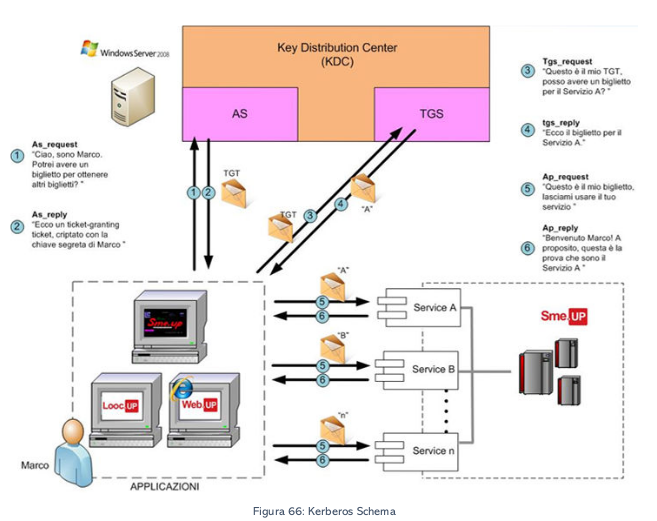
\includegraphics[width=7cm, keepaspectratio]{Bistarelli/img/keberos/keberos1.png}
\end{figure}

\begin{figure}[H]
	\centering
    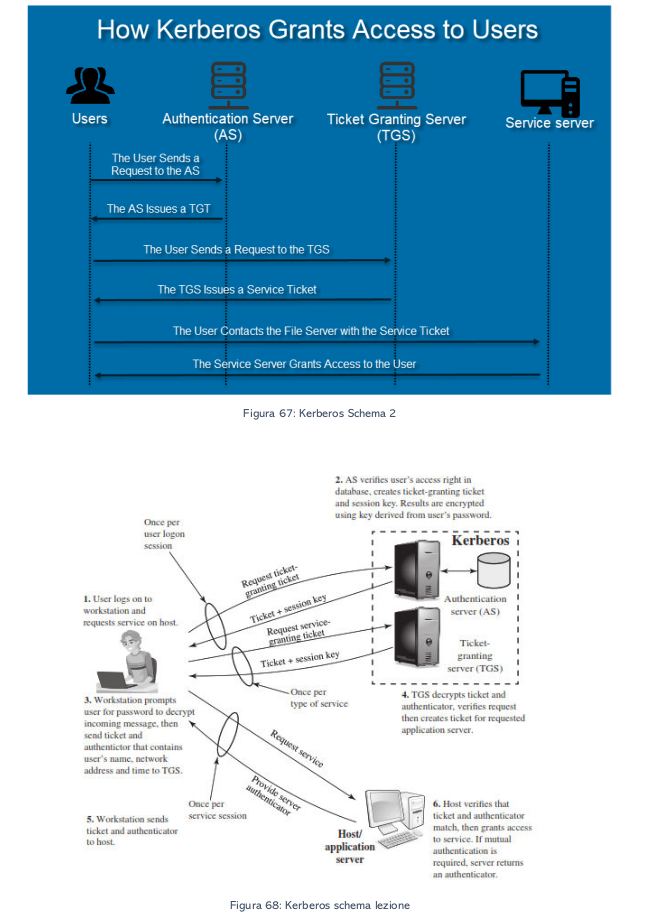
\includegraphics[width=7cm, keepaspectratio]{Bistarelli/img/keberos/keberos2.png}
\end{figure}

\subsection{Caratteristiche}
\begin{itemize}
    \item 3 fasi: autenticazione, autorizzazione, servizio
    
    \item Ultime 2 opzionali e trasparenti all’utente
    
    \item Ognuna fornisce credenziali per successiva
    
    \begin{itemize}
        \item Fase 1 fornische authKey e authTicket per la 2
        
        \item Fase 2 fornisce servKey e servTicket per la fase 3
    \end{itemize}
    
    \item Ogni tipo di chiave si sessione ha sua durata (in genere quelle per i servizi dura meno, es. sessione 1 giorno, servizio 1 ora)
    
    \item Una authKey può criptare divere servKey
    
\end{itemize}
\textbf{Nota:} Chiave pubblica e privata per autenticazione, chiave di sessione per la sessione (authKey e servKey)
perché ha una durata limitata e servono a dare confidentiality/confidenzialità a questa comunicazione in modo da
cifrarla.

\begin{figure}[H]
	\centering
    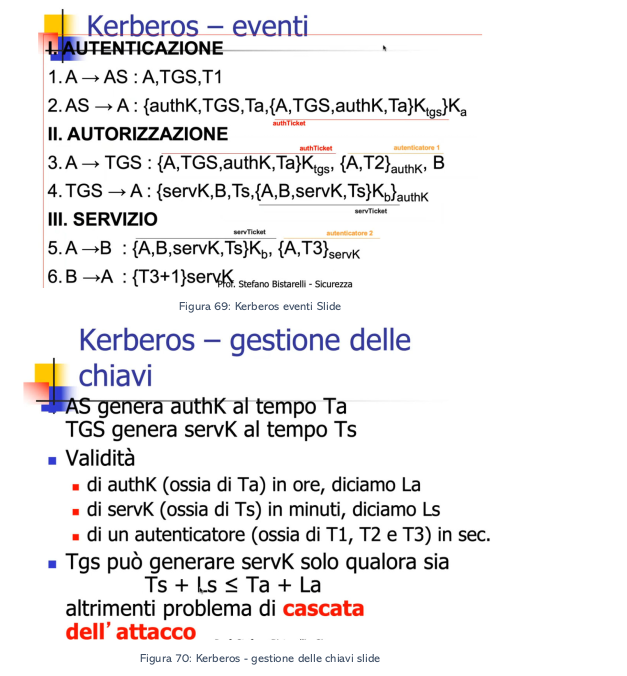
\includegraphics[width=7cm, keepaspectratio]{Bistarelli/img/keberos/keberos3.png}
\end{figure}

\begin{figure}[H]
	\centering
    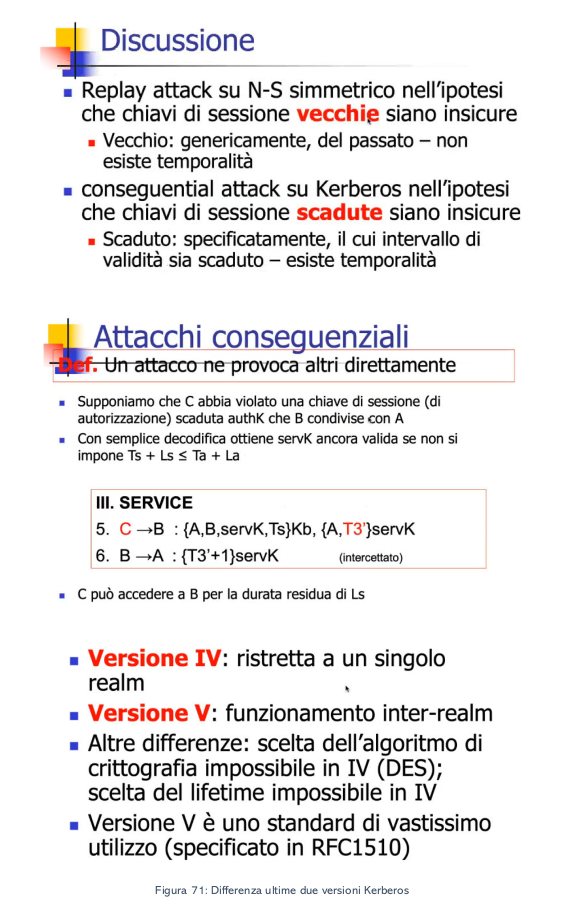
\includegraphics[width=7cm, keepaspectratio]{Bistarelli/img/keberos/keberos4.png}
\end{figure}

\begin{figure}[H]
	\centering
    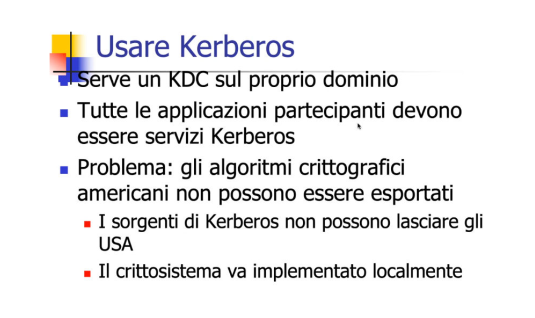
\includegraphics[width=7cm, keepaspectratio]{Bistarelli/img/keberos/keberos5.png}
\end{figure}
\subsection{Descrizione del protocollo}
Il client si autentica \textbf{sull'Authentication Server (AS)} che inoltra il nome utente a un centro di distribuzione
delle chiavi (KDC) . Il KDC emette un \textbf{ticket-granting ticket (TGT)} , che è timestamp e lo crittografa utilizzando la chiave segreta del \textbf{ticket-granting service (TGS)} e restituisce il risultato crittografato alla workstation dell'utente. Questa operazione viene eseguita raramente, in genere all'accesso dell'utente; il TGT scade a un certo punto sebbene possa essere rinnovato in modo trasparente dal gestore della sessione dell'utente mentre è
connesso. Quando il client ha bisogno di comunicare con un servizio su un altro nodo (un "principal", nel gergo
Kerberos), il client invia il \textbf{TGT} al \textbf{TGS}, che di solito condivide lo stesso host del KDC. Il servizio deve essere già stato registrato con il TGS con un nome dell'entità servizio (SPN) . Il client utilizza l'SPN per richiedere l'accesso a questo servizio. Dopo aver verificato che il TGT è valido e che l'utente è autorizzato ad accedere al servizio richiesto, il TGS emette il ticket e le chiavi di sessione al client. Il client invia quindi il ticket al \textbf{server del servizio (SS)} insieme alla sua richiesta di servizio.

\begin{figure}[H]
	\centering
    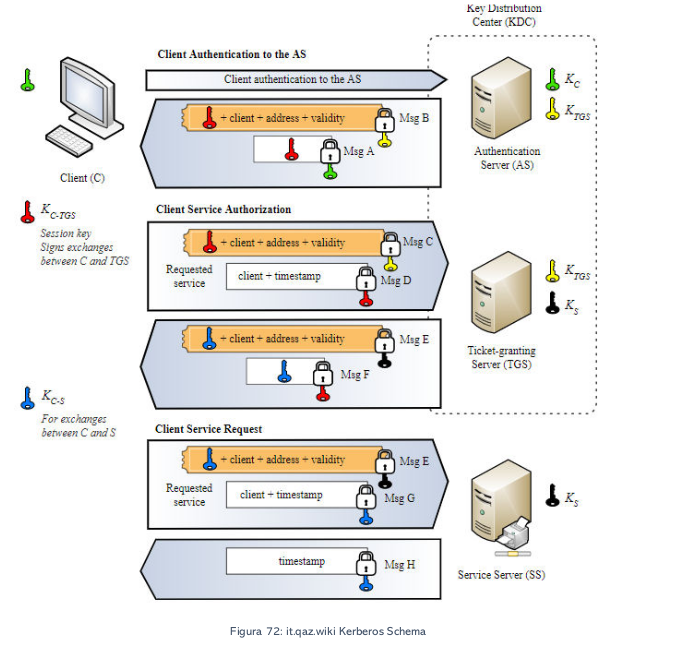
\includegraphics[width=7cm, keepaspectratio]{Bistarelli/img/keberos/keberos6.png}
\end{figure}
\subsection{Accesso basato su client utente}
Un utente immette un nome utente e una password sui computer client . Altri meccanismi di credenziali come
pkinit ( RFC 4556 ) consentono l'uso di chiavi pubbliche al posto di una password. Il client trasforma la password
nella chiave di un cifrario simmetrico. Questo utilizza la pianificazione della chiave incorporata o un hash
unidirezionale , a seconda della suite di crittografia utilizzata.
\subsection{Autenticazione client}
\begin{enumerate}
    \item Il client invia un messaggio di testo in chiaro dell'ID utente all'AS (Authentication Server) richiedendo servizi per conto dell'utente. (Nota: né la chiave segreta né la password vengono inviate all'AS.)
    
    \item L'AS verifica se il client è nel suo database. In tal caso, l'AS genera la chiave segreta eseguendo l'hashing della password dell'utente trovata nel database (ad esempio, Active Directory in Windows Server) e restituisce i seguenti due messaggi al client:
    
    \begin{itemize}
        \item Messaggio A: chiave di sessione client / TGS crittografata utilizzando la chiave segreta del client/ utente.
        
        \item Messaggio B: Ticket-Granting-Ticket (TGT, che include l'ID client, l' indirizzo di rete del client , il periodo di validità del ticket e la chiave di sessione client / TGS ) crittografato utilizzando la chiave segreta del TGS.
    \end{itemize}
    
    \item Una volta che il client riceve i messaggi A e B, tenta di decrittografare il messaggio A con la chiave segreta generata dalla password inserita dall'utente. Se la password inserita dall'utente non corrisponde alla password nel database AS, la chiave segreta del client sarà diversa e quindi non sarà in grado di decifrare il messaggio A. Con una password e una chiave segreta valide il client decrittografa il messaggio A per ottenere la chiave di sessione client / TGS . Questa chiave di sessione viene utilizzata per ulteriori comunicazioni con il TGS. (Nota: il client non può decrittografare il messaggio B, poiché è crittografato utilizzando la chiave segreta del TGS.) A questo punto, il client dispone di informazioni sufficienti per autenticarsi al TGS.
\end{enumerate}
\subsection{Autenticazione del servizio clienti}
\begin{enumerate}
    \item Quando richiede servizi, il client invia i seguenti messaggi al TGS:
    
    \begin{itemize}
        \item Messaggio C: composto dal messaggio B (il TGT crittografato che utilizza la chiave segreta TGS) e dall'ID del servizio richiesto.
        
        \item Messaggio D: Autenticatore (composto dall'ID client e dal timestamp), crittografato utilizzando la chiave di sessione client / TGS
    \end{itemize}
    
    \item Alla ricezione dei messaggi C e D, il TGS recupera il messaggio B dal messaggio C. Decrittografa il messaggio B utilizzando la chiave segreta TGS. Questo fornisce la "chiave di sessione client / TGS" e l'ID client (entrambi sono nel TGT). Utilizzando questa "chiave di sessione client / TGS", il TGS decrittografa il messaggio D (Authenticator) e confronta gli ID client dai messaggi B e D; se corrispondono, il server invia i seguenti due messaggi al client:
    
    \begin{itemize}
        \item Messaggio E: ticket da client a server (che include ID client, indirizzo di rete client, periodo di validità e chiave di sessione client / server ) crittografato utilizzando la chiave segreta del servizio.
        
        \item Messaggio F: chiave di sessione client / server crittografata con chiave di sessione client / TGS.
    \end{itemize}
\end{enumerate}
\subsection{Richiesta di servizio clienti}
\begin{enumerate}
    \item Dopo aver ricevuto i messaggi E ed F da TGS, il client dispone di informazioni sufficienti per autenticarsi al Service Server (SS). Il client si connette alla SS e invia i seguenti due messaggi:
    
    \begin{itemize}
        \item Messaggio E: dal passaggio precedente (il ticket da client a server , crittografato utilizzando la chiave segreta del servizio).
        
        \item Messaggio G: un nuovo autenticatore, che include l'ID client, il timestamp ed è crittografato utilizzando la chiave di sessione client / server.
    \end{itemize}
    
    \item L'SS decrittografa il ticket (messaggio E) utilizzando la propria chiave segreta per recuperare la chiave di sessione client / server . Utilizzando la chiave delle sessioni, SS decrittografa l'Autenticatore e confronta l'ID client dai messaggi E e G, se corrispondono, il server invia il seguente messaggio al client per confermare la sua vera identità e disponibilità a servire il client:
    
    \begin{itemize}
        \item Messaggio H: il timestamp trovato nell'autenticatore del client (più 1 nella versione 4, ma non necessario nella versione 5), crittografato utilizzando la chiave di sessione client / server.
    \end{itemize}
    
    \item Il client decrittografa la conferma (messaggio H) utilizzando la chiave di sessione client / server e controlla se il timestamp è corretto. In tal caso, il client può considerare attendibile il server e può iniziare a inviare richieste di servizio al server.
    
    \item Il server fornisce i servizi richiesti al client.
\end{enumerate}
\subsection{Inconvenienti e limitazioni}
\begin{itemize}
    \item Kerberos ha requisiti di tempo rigorosi, il che significa che gli orologi degli host coinvolti devono esseresincronizzati entro i limiti configurati. I ticket hanno un periodo di disponibilità temporale e se l'orologiodell'host non è sincronizzato con l'orologio del server Kerberos, l'autenticazione fallirà. La configurazione predefinita per MIT richiede che gli orari dell'orologio non siano distanti più di cinque minuti. In pratica , i demoni Network Time Protocol vengono solitamente utilizzati per mantenere sincronizzati gli orologi host. Si noti che alcuni server (l'implementazione di Microsoft è uno di questi) possono restituire un risultato KRB\_AP\_ERR\_SKEW contenente l'ora del server crittografata nel caso in cui entrambi gli orologi abbiano un offset maggiore del valore massimo configurato. In tal caso, il client potrebbe riprovare calcolando l'ora utilizzando l'ora del server fornita per trovare l'offset. Questo comportamento è documentato in RFC 4430.
    
    \item Il protocollo di amministrazione non è standardizzato e differisce tra le implementazioni del server. Le modifiche alla password sono descritte in RFC 3244
    
    \item In caso di adozione della crittografia simmetrica (Kerberos può funzionare utilizzando la crittografia simmetrica o asimmetrica (chiave pubblica)), poiché tutte le autenticazioni sono controllate da un centro di distribuzione delle chiavi centralizzato (KDC), la compromissione di questa infrastruttura di autenticazione consentirà a un utente malintenzionato di impersonare qualsiasi utente
    
    \item Ogni servizio di rete che richiede un nome host diverso avrà bisogno del proprio set di chiavi Kerberos. Ciò complica l'hosting virtuale e i cluster.
    
    \item Kerberos richiede che gli account utente e i servizi abbiano una relazione affidabile con il server di token Kerberos.
    
    \item La fiducia del client richiesta rende difficile la creazione di ambienti a fasi (ad esempio, domini separati per l'ambiente di test, l'ambiente di pre-produzione e l'ambiente di produzione): è necessario creare relazioni di fiducia del dominio che impediscano una netta separazione dei domini dell'ambiente o che siano necessari client utente aggiuntivi previsto per ogni ambiente.
\end{itemize}
\subsection{Vulnerabilità}
La crittografia Data Encryption Standard (DES) può essere utilizzata in combinazione con Kerberos, ma non è più uno standard Internet perché è debole. Esistono vulnerabilità di sicurezza in molti prodotti legacy che implementano Kerberos perché non sono stati aggiornati per utilizzare crittografie più recenti come AES invece di DES. Nel novembre 2014, Microsoft ha rilasciato una patch (MS14-068) per correggere una vulnerabilità sfruttabile nell'implementazione Windows del Kerberos Key Distribution Center (KDC). La vulnerabilità presumibilmente consente agli utenti di "elevare" (e abusare) i propri privilegi, fino al livello di dominio.
\subsection{Altra descrizione del protocollo (wikipedia)}
In informatica e telecomunicazioni Kerberos è un protocollo di rete per l'autenticazione forte che permette a diversi
terminali di comunicare su una rete informatica insicura provando la propria identità mediante l'utilizzo di tecniche
di crittografia simmetrica. Kerberos previene attacchi quali l'intercettazione e i replay attack ed assicura l'integrità
dei dati. I suoi progettisti mirarono soprattutto ad un modello client-server, e fornisce una mutua autenticazione
cioè sia l'utente sia il fornitore del servizio possono verificare l'identità dell'altro.
\subsubsection{Descrizione}
Kerberos si basa sul protocollo di Needham-Schroeder. Utilizza una terza parte affidabile per centralizzare la
distribuzione delle chiavi detta Key Distribution Center (KDC), che consiste di due parti separate logicamente:
l'Authentication Server (AS) e il Ticket Granting Server (TGS). Kerberos funziona utilizzando dei "biglietti" (detti
ticket) che servono per provare l'identità degli utenti.

\singlespacing

L'AS mantiene un database delle chiavi segrete; ogni entità sulla rete — che sia un client o un server — condivide
la chiave segreta solo con l'AS. La conoscenza di questa chiave serve per provare l'identità di un'entità. Per
comunicazioni tra due entità, Kerberos genera una chiave di sessione, che può essere utilizzata dai due terminali
per comunicare.

\subsubsection{Il protocollo}
Il protocollo può essere definito come segue utilizzando la notazione per protocolli di sicurezza, dove Alice (A) si
autentica presso Bob (B) usando il server S:

\begin{figure}[H]
	\centering
    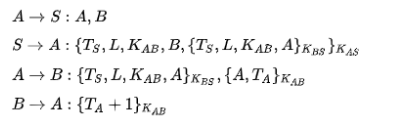
\includegraphics[width=7cm, keepaspectratio]{Bistarelli/img/keberos/keberos7.png}
\end{figure}

La sicurezza del protocollo si basa fortemente sui timestamp T e sui tempi di vita L come indicatori affidabili della
creazione recente della comunicazione per evitare replay attack (vedi logica BAN).

\singlespacing

È importante notare come il server S stia sia come Authentication Service (AS) sia come Ticket Granting Service
(TGS).

\begin{figure}[H]
	\centering
    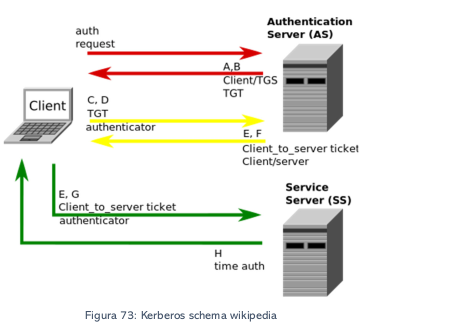
\includegraphics[width=7cm, keepaspectratio]{Bistarelli/img/keberos/keberos8.png}
\end{figure}
\subsubsection{Operazioni di Kerberos}
Quella che segue è una descrizione semplificata del protocollo. Saranno utilizzate le seguenti abbreviazioni: AS =
Authentication Server, TGS = Ticket Granting Server, SS = Service Server.In breve: il client si autentica presso AS
che gli fornisce un ticket di sessione per accedere a TGS, si autentica presso TGS e riceve il ticket per aprire una
sessione di comunicazione con SS. In dettaglio
\subsubsection{Utente: autenticazione di base}
\begin{enumerate}
    \item Un utentie inserisce username e password sul client
\end{enumerate}
\subsubsection{Client: Autenticazione AS}
\begin{enumerate}
    \item Il client manda un messaggio non criptato all'AS richiedendo i servizi per l'utente. ("L'utente XYZ vorrebbe richiedere dei servizi"). Né la chiave segreta né la password vengono inviate all'AS.
    
    \item L'AS controlla se il client è nel suo database. Se lo è invia due messaggi al client:
    
    \begin{itemize}
        \item Messaggio A: Chiave di sessione client-TGS criptata usando la chiave segreta dell'utente.
        
        \item Messaggio B: Ticket-Granting Ticket (che include l'identificativo del client, l'indirizzo di rete, il tempo di validità del ticket e la chiave di sessione client-TGS). Il Ticket-Granting Ticket è criptato utilizzando la chiave segreta di TGS.
    \end{itemize}
    
    \item Quando il client riceve i messaggi A e B, decripta il messaggio A ottenendo la chiave di sessione client-TGS. Questa chiave è utilizzata per le successive comunicazioni con TGS. (Nota: il client non può decriptare il Messaggio B, che è stato criptato con la chiave segreta di TGS). A questo punto il client possiede i mezzi per autenticarsi presso TGS.
\end{enumerate}
\subsubsection{Client: Autenticazione TGS}
\begin{enumerate}
    \item Quando richiede dei servizi, il client invia i seguenti due messaggi a TGS:
    \begin{itemize}
        \item Messaggio C: composto dal Ticket-Granting Ticket (mandatogli dal AS nel messaggio B) e dall'identificativo del servizio richiesto
        
        \item Messaggio D: autenticatore (Authenticator) (che è formato da identificativo del client e imestamp), criptato usando la chiave di sessione client—TGS.
    \end{itemize}
    \item Ricevendo i messaggi C e D, TGS decripta il messaggio C con la propria chiave e dal messaggio estrae la chiave di sessione client—TGS che utilizza per decriptare il messaggio D (autenticatore). A questo punto invia i seguenti due messaggi al client:
    \begin{itemize}
        \item Messaggio E: Ticket client-server (che include l'identificativo del client, l'indirizzo di rete del client, il periodo di validità e la chiave di sessione client-server) criptato utilizzando la chiave segreta del server che offre il servizio.
        
        \item Messaggio F: Chiave di sessione client-server criptato usando la chiave di sessione client-TGS
    \end{itemize}
\end{enumerate}
\subsubsection{Client: Autenticazione SS}
\begin{enumerate}
    \item Ricevendo i messaggi E e F dal TGS, il client può autenticarsi presso il SS. Il client si connette al SS e invia i seguenti due messaggi:
    
    \begin{itemize}
        \item Messaggio E: Ticket client-server criptato usando la chiave segreta di SS.
        
        \item Messaggio G: un nuovo autenticatore, che include l'identificativo del client, il timestamp ed è
    \end{itemize}
    
    \item Il server decripta il ticket usando la sua chiave segreta e invia il seguente messaggio al client per confermare la propria identità e la volontà di fornire il servizio al client:
    
    \begin{itemize}
        \item Messaggio H: il timestamp trovato nell'autenticatore incrementato di uno, criptato utilizzando la chiave di sessione client-server.
    \end{itemize}
    
    \item Il client decripta la conferma usando la chiave di sessione client-server e controlla che il timestamp sia correttamente aggiornato. Se lo è, il client può considerare affidabile il server e iniziare a effettuare le richieste di servizio.
    
    \item Il server fornisce i servizi al client.
    
    
\end{enumerate}